\chapter{State-of-the-Art} \label{chap:sota}

\section*{}

\section{Introduction}
In order to find the best approach to this problem, some research on already existing methodologies and concepts was needed. First an overview for the general categories researched is given, followed by the actual state of the art found, divided by relevant subcategories. 

\section{Reverse Engineering}\label{sec:reverseengineering}

Reverse engineering is “the process of analyzing the subject system to identify the system components and interrelationships and to create representations of the system in another form or at a higher level of abstraction” \cite{chikofsky1990reverse}.

There are two methods of applying reverse engineering to a system: the dynamic method, in which the data are retrieved from the system at run time without access to the source code, and the static method, which obtains the data from the system source code \cite{systa1999dynamic}. There is also the hybrid method, which combines the two previous methods, and the historical method, which includes historic information to see the evolution of the software system \cite{canfora2011achievements}. These approaches follow the same main steps: collect the data, analyse it and represent it in a legible way, and in the process allow the discovery of information about the system's control and data flow \cite{pacione2003comparative}.

\subsection{Extraction of Information from Execution Traces} \label{sec:extractexecutiontraces}

Plenty of approaches that extract information from execution traces have been found. Elbaum \cite{elbaum2003improving} presents a testing approach that utilizes data captured in user sessions to create test cases. Duarte, Kramer and Uchitel defined an approach for behavior model extraction which combines static and dynamic information \cite{duarte2006model}. Sampath \textit{et al.} developed an approach for achieving scalable user-session-based testing of web applications, that applies concept analysis for clustering user sessions and a set of heuristics for test case selection \cite{sampath2007applying}. TraceServer \cite{andjelkovic2011trace} is an extension of the Java PathFinder model checking tool \cite{jpf} which collects and analyzes execution traces. jRapture \cite{steven2000jrapture} is a technique and a tool for capture and replay of Java program executions. ReGUI \cite{coimbra2011reverse,coimbra2012dynamic} is a dynamic reverse engineering tool made to reduce the effort of modeling the structure and behavior of a software application GUI.  Fischer \textit{et al.} developed a methodology that analyzes and compares execution traces of different versions of a software system to provide insights into its evolution, named EvoTrace \cite{fischer2005system}. Amalfitano's approach \cite{amalfitano2010rich} generates test cases from execution traces to help testing from Rich Internet Applications (RIAs), with the execution traces being obtained from user sessions and crawling the application. 

\subsection{Extraction of Information from Web Applications}

The following approaches extract information from Web applications for analysis and processing. 

Ricca and Tonella's ReWeb \cite{ricca2001understanding} dynamically extracts information from a Web application's server logs to analyze its structure and evolution, and so aims to find inconsistencies and connectivity problems. Benedikt \textit{et al.} introduced a framework called VeriWeb \cite{benedikt2002veriWeb} that discovers and explores automatically Web-site execution paths that can be followed by a user in a Web application. Di Lucca \textit{et al.}'s approach \cite{di2005integrating} integrates WARE \cite{di2004reverse}, a static analysis tool that generates UML diagrams from a Web application's source code, and WANDA \cite{antoniol2004understanding}, a Web application dynamic analysis tool, to identify groups of equivalent built client pages and to enable a better understanding of the application under study. Bernardi \textit{et al.} \cite{bernardi2008reverse} presents an approach for the semi-automatic recovery of user-centered conceptual models from existing web aplications, where the models represents the application's contents, their organization and associations, from a user-centered perspective. Marchetto \textit{et al.} proposed a state-based Web testing approach \cite{marchetto2008state} that abstracts the Document Object Model (DOM) into a state model, and from the model derives test cases. Crawljax \cite{roest2010automated} is a tool that obtains graphical site maps by automatically crawling through a Web application. WebDiff \cite{choudhary2010Webdiff} is a tool that searches for cross-browser inconsistencies by analyzing a website's DOM and comparing screenshots obtained in different browsers. Memon presented an end-to-end model-based Web application automated testing approach \cite{memon2007event} by consolidating previous model development work into one general event-flow model, and employs three ESESs (event space exploration strategies) for model checking, test-case generation, and test-oracle creation. Mesbah \textit{et al.} proposed an automated technique for generating test cases with invariants from models inferred through dynamic crawling \cite{mesbah2012invariant}. Artzi \textit{et al.} developed a tool called Artemis \cite{artzi2011framework} which performs feedback-directed random test case generation for Javascript Web applications. Artemis triggers events at random, but the events are prioritized by less covered branch coverage in previous sequences. Amalfitano \textit{et al.} developed a semi-automatic approach \cite{amalfitano2011using} that uses dynamic analysis of a Web application to generate end user documentation, compliant with known standards and guidelines for software user documentation. Dincturk \textit{et al.} \cite{dincturk2012statistical} proposed a RIA crawling strategy using a statistical model based on the model-based crawling approach introduced in \cite{benjamin2011strategy} to crawl RIAs efficiently. Another approach by Mesbah \textit{et al.}, named FeedEx \cite{fard2013feedback} is a feedback-directed Web application exploration technique to derive test models. It uses a greedy algorithm to partially crawl a RIA's GUI, and the goal is that the derived test model capture different aspects of the given Web application's client-side functionality.  Dallmeier \textit{et al.}'s Webmate \cite{dallmeier2012Webmate,dallmeier2013Webmate} is a tool that analyzes the Web application under test, identifies all functionally different states, and is then able to navigate to each of these states at the user’s request.

\subsection{Inferring Patterns from Web applications}
Despite the fact that there are plenty of approaches to mine patterns from Web applications, no approaches have been found that infer UI patterns from Web applications beside the work this thesis means to extend \cite{nabuco2013inferring, morgado2012gui}. The approaches found deal mostly with Web mining, with the goal of finding relationships between different data or finding the same data in different formats. Brin \cite{brin1999extracting} presented an approach to extract relations and patterns for the same data spread through many different formats. Chang \cite{chang2003automatic} proposes a similar method to discover patterns, by extracting structured data from semi-structured Web documents. Freitag \cite{freitag1998information} proposed a general-purpose relational learner for information extracting from Web applications.

\subsection{Capture-Replay Tools}
The execution traces of a Web application, on the client side, are usually captured via a capture-replay tool. Here we present the most popular capture-replay tools used nowadays.

Selenium \footnote{Selenium: \url{http://docs.seleniumhq.org/}} is an open-source capture/replay tool that captures an user's interaction with a Web application in HTML files. It has multi browser, OS and language support, can be installed server-side and as a Mozilla Firefox add-on, has its own IDE \textit{(Integrated Development Environment)}, and allows recording and playback of tests.

Watir Webdriver \footnote{Watir: \url{http://watirwebdriver.com/}} is is an open-source (BSD) family of Ruby libraries for automating Web browsers and Web application testing. It has multi browser and OS support, a rich API, and has a functionality for non-tech users: the ‘Simple’ class. There also exist ports for other programming languages, such as Watij (for Java) and Watin (.NET).

IBM Rational Functional Tester (RFT) \footnote{IBM RFT: \url{http://www-03.ibm.com/software/products/en/functional}} is an automated functional testing and regression testing tool. This software provides automated testing capabilities for functional, regression, GUI, and data-driven testing. Rational Function Tester supports a range of applications, such as .Net, Java, Siebel, SAP, terminal emulator-based applications, PowerBuilder, Ajax, Adobe Flex, and others. It permits storyboard testing, automated testing, data-driven testing, and test scripting.

Sahi \footnote{Sahi: \url{http://sahi.co.in/}} is an open-source automation and testing tool for web applications. It allows recording and replaying across browsers, provides different language drivers for writing test scripts, and supports Ajax and highly dynamic web applications. 

\section{Data Mining}\label{sec:datamining}

Data mining is \textit{“(...) the non-trivial extraction of previously unknown and potentially useful information from data”} \cite{fayyad1996data}. It is the analysis step of a Knowledge Discovery in Databases (KDD) process, and an interdisciplinary sub-field of computer science. It combines artificial intelligence, machine learning, statistics and database systems \cite{chakrabarti2004data}.

The goal of data mining is to extract information from a dataset, or past data, and transform it into an understandable structure. Discovering information from data takes two major forms: \textbf{description} (finding human-interpretable patterns describing the data) and \textbf{prediction} (using some variables to predict unknown or future values of other variables) \cite{maimon2005data}. Common types of data mining analysis include:
\begin{description}
	\item[Anomaly detection] (can also be called outlier/change/deviation detection) involves getting a sense of the typical cases that the dataset tends to contain, to better detect cases that are different from the regular pattern.
	\item[Association learning] aim to find correlations between different attributes in a dataset.
	\item[Cluster detection] is the task of discovering groups and structures in the data that are in some way or another "similar", without using known structures in the data.
	\item[Classification] classifies new cases based on pre-determined categories. Learning from a large set of pre-classified examples, algorithms can detect systematic differences between items in each group and apply these corresponding models to new classification problems.
	\item[Regression] aims to fit an equation into a dataset, in order to predict one or more continuous variables, such as profit or loss, based on other attributes in the dataset.
\end{description}

The performance of an algorithm depends greatly on the characteristics of the data. There is no single algorithm that works best on all given problems \cite{wolpert1995no} so in the interest of determining the best approach, the best choice is to try a wide variety and then compare their results.
% TODO - FINISH %%%%%%%%%%%%%%%%%%%%%%%%%%%%%%%%%%%%%%%%%%%%%%%%%

\subsection{Data Mining Algorithm Categories}\label{sec:dmalgorithms}
In this project we will be concerned with the association and sequence mining side of data mining. Below, we will review some algorithms that can be used in these kinds of problems.

\subsubsection{Association Rules}
Association rule learning is a method for discovering interesting relations between variables in large databases. It is intended to identify strong rules discovered in databases using different measures of interestingness \cite{han2006data}. Association rules are employed today in many application areas including Web usage mining, intrusion detection, continuous production, and bioinformatics. Association rules have the form 

\begin{equation}Body \rightarrow Head\;[support, confidence]\end{equation} 

(for a definition of support and confidence, please check Section \ref{sec:metrics}). Association rule mining can be broadly classified into categories: \textbf{boolean} or \textbf{quantitative} associations, \textbf{single dimension} or \textbf{multidimensional} associations, \textbf{single level} or \textbf{multilevel} associations. As opposed to sequence mining, association rule learning typically does not consider the order of items either within a transaction or across transactions. 

To better explain these categories, we present two equations: 
\begin{equation}\label{eq:eq1} buys(x, SQLServer) \cap buys(x, DMBook) \rightarrow buys(x, DBMiner\;[5\%, 65\%]\end{equation} and 
\begin{equation}\label{eq:eq2} age(x, [30..39]) \cap income(x, [42..50]) \rightarrow buys(x, PC)\;[1\%, 75\%]\end{equation}


\textbf{Boolean} and \textbf{quantitative} association rules difer mainly on the type of values handled (for example, equation \ref{eq:eq1} is a boolean rule, while equation \ref{eq:eq2} is a quantitative rule). \textbf{Single dimension} and \textbf{multidimensional} association rules difer in the number of dimensions/predicates employed in the rule (the equation \ref{eq:eq1} is a single-dimension rule, since it only uses one dimension (\textit{buys}) while the equation \ref{eq:eq2} is multidimensional because it includes three dimensions, \textit{age}, \textit{income}, and \textit{buys}). 

A notable and popular association rule algorithm is the \textbf{Apriori} algorithm \cite{wu2008top}. \textbf{Apriori} is a seminal algorithm for finding frequent itemsets using candidate generation \cite{agrawal1994fast}. It is characterized as a level-wise complete search algorithm using anti-monotonicity of itemsets, “if an itemset is not frequent, any of its superset is never frequent”. By convention, Apriori assumes that items within a transaction or itemset are sorted in lexicographic order. Apriori first scans the database and searches for frequent itemsets of size 1 by accumulating the count for each item and collecting those that satisfy the minimum support requirement. It then iterates on the following three steps and extracts all the frequent itemsets. Ergo, Apriori uses a "bottom up" approach, where frequent subsets are extended one item at a time (a step known as \textit{candidate generation}), and groups of candidates are tested against the data. The algorithm terminates when no further successful extensions are found.

\subsubsection*{Frequent patterns without candidate generation} 
As mentioned before, Apriori includes a step called “candidate generation”, in which itemsets are generated and extended iteratively.  However, candidate set generation is costly, especially when there exist prolific patterns and/or long patterns \cite{han2000mining}. The \textbf{FP-growth} algorithm uses the frequent pattern tree (FP-tree) structure to mine the complete set of frequent patterns by pattern fragment growth. 

\subsubsection*{Multilevel association rules}

\subsubsection*{Correlation rules}

\subsubsection*{Sequential rules}

\begin{description}
\item[Sequential rule mining with window constraint]
\item[Sequential rule mining]
\item[Top-k sequential rule mining]
\item[Top-k non-redundant sequential rule mining]
\end{description}

\subsubsection{Sequential Pattern Mining}
Sequence mining is a topic of Data Mining concerned with finding statistically relevant patterns between data examples where the values are delivered in a sequence. A \textbf{sequential pattern} is a sequence of item sets that occur frequently in a specific order, within a certain time gap. An example of a sequence could be transactions made by a customer, with

\subsubsection*{Apriori-based approaches} 

There are two algorithms in this category: \textbf{GSP} (Generalized Sequential Pattern) algorithm and the \textbf{SPADE} algorithm. 

\textbf{GSP} Algorithm (Generalized Sequential Pattern algorithm) is an algorithm used for sequence mining. The algorithms for solving sequence mining problems are mostly based on the a priori (level-wise) algorithm. One way to use the level-wise paradigm is to first discover all the frequent items in a level-wise fashion, counting the occurrences of all singleton elements in the database. Afterwards, the non-frequent items are removed. At the end of this step, each transaction consists of only the frequent elements it originally contained. This modified database becomes an input to the GSP algorithm. This process requires one pass over the whole database. 

\textbf{SPADE} is a fundamentally different sequential pattern algorithm. In place of repeated database scans, this method uses lattice-search techniques and simple join operations to discover all sequence patterns. First a vertical id-list is created to associate with each item, a list of the sequences in which it occurs, along with the appropriate time-stamps. 

\subsubsection*{Pattern-growth based approaches} 

There are two algorithms in this category: \textbf{FreeSpan} and \textbf{PrefixSpan}.

\textbf{FreeSpan} was developed to substantially reduce the expensive candidate generation and testing of Apriori, while maintaining its basic heuristic. In general, FreeSpan uses frequent items to recursively project the sequence database into projected databases while growing subsequence fragments in each projected database. Each projection partitions the database and confines further testing to progressively smaller and more manageable units. The trade-off is a considerable amount of sequence duplication, as the same sequence could appear in more than one projected database. However, the size of each projected database usually (but not necessarily) decreases rapidly with recursion. 

\textbf{Prefix Span} was developed to address the costs of Free Span. Its general idea is that, instead of projecting sequence databases by considering all the possible occurrences of frequent subsequences, the projection is based only on frequent prefixes because any frequent subsequence can always be found by growing a frequent prefix. 

\subsubsection*{Closed sequential pattern mining}
Sequential pattern mining mine the full set of frequent subsequences satisfying the \textit{minsup} threshold. However, since frequent long sequences contains a combination of frequent subsequences, the process will generate an explosion of frequent subsequences \cite{yan2003clospan}. Closed sequential pattern mining mines \textit{frequent closed sequences} (sequences that contain no super-sequence with the same support) instead. For a definition of \textit{support} see Equation \ref{eq:support}. This kind of sequence mining produces significantly less sequences than the alternative while preserving the same expressive power \cite{yan2003clospan}.

\subsubsection*{Multi-dimensional sequential pattern mining}
Generally, sequential pattern algorithms mine only one dimension. This is fine if the transaction dataset to mine is also unidimensional (simple transactions with timestamps associated) but usually sequence patterns are associated with different circumstances (for example, customer purchases can be associated with region, customer group, date, and others). When one or more dimensions of information is mined and the order of the dimension values is not important, it is known as multi-dimensional sequential pattern mining \cite{pinto2001multi}. The goal of multidimensional sequential pattern mining is to cover more useful information than 
regular sequential patterns.

\subsubsection*{Closed Multi-dimensional sequential pattern mining}
Multidimensional sequencial pattern mining generally produce a large set of redundant patterns \cite{songram2008closed}. Since the problem of redundancy is similar to those of itemset pattern mining and sequential pattern mining, the combination of closed itemset pattern mining and closed sequential pattern mining returns closed multidimensional sequential patterns (or CMDS patterns). This method consists of two major steps; (1) combination closed itemset pattern mining with closed sequential pattern mining, and (2) elimination of redundant patterns.

\subsubsection{Evaluation Metrics}\label{sec:metrics}
Below are presented some metrics used for evaluating association rules.

\begin{description}
	\item[Itemset.] An itemset is a collection of one or more items. It can also be called k-itemset, where k is its size.
	\item[Support count.] The support count of an itemset is defined as its frequency of occurrence. 
	\item[Support.] The support of an itemset is the fraction of transactions that contain the itemset (see Equation \ref{eq:support}). 
		\begin{equation}\label{eq:support}
			supp(X) =\frac{itemset\_occurrences(X)}{all\_transactions}
		\end{equation}
	\item[Confidence.] Confidence is the support for occurrences of transactions where X and Y both appear (see Equation \ref{eq:confidence}). 
		\begin{equation}\label{eq:confidence}
			conf(X \Rightarrow Y) =\frac{supp(X \cap Y)}{supp(X)}
		\end{equation}
	\item[Frequent itemset.] A frequent itemset is one with support count equal or superior to the \textit{minsup} threshold, the minimum number of occurrences specified by the user.
	\item[Lift.] Lift is the ratio of the observed support to that expected if X and Y were independent (see Equation \ref{eq:lift}). 
		\begin{equation} \label{eq:lift}
			lift(X \Rightarrow Y)=\frac{supp(X \cup Y)}{supp(X) \times supp(Y)}
		\end{equation}
	\item[Conviction.] Conviction  can be interpreted as the ratio of the expected frequency that X occurs without Y (that is to say, the frequency that the rule makes an incorrect prediction) if X and Y were independent divided by the observed frequency of incorrect predictions (see Equation \ref{eq:conviction}). In sum, it measures the degree of independence between two variables.
		\begin{equation} \label{eq:conviction}
			 conv(X \Rightarrow Y)=\frac{1-supp(Y)}{1-conf(X\Rightarrow Y)}
		\end{equation}
\end{description}
\subsection{Data Mining Tools and Frameworks}\label{sec:dmtools}
Except in rare cases of very specific problems, it typically makes no sense for someone to implement any data mining algorithm that they might need. There are many data mining tools (many of which free) that already implement many of those algorithms and have customization capabilities that make it easy to adapt them to most problems; and there are also many data mining frameworks and libraries who implement a wide variety of algorithms. A data mining tool is a powerful software that makes use of data mining algorithms, and supports a complete KDD process \cite{mikut2011data}. In the following sections we will briefly address some of the most commonly used open-source tools and frameworks, namely RapidMiner, WEKA, SPMF, and R. 

\subsubsection{RapidMiner}
RapidMiner \footnote{RapidMiner: \url{http://www.rapidminer.com}} is a complete solution for data mining problems. It’s available as a standalone GUI based application, as seen in Figure \ref{fig:rapidminer}. It is a commercial application, although its core and earlier versions are distributed under an open source license, and it offers a free version, beyond its multiple paid versions. Being one of the most popular data mining tools used today, its applications span several domains, including education, training, industrial and personal applications, among others. Its functionality can also be easily extended through the use of plugins. reflecting in an increased value for this tool.

\begin{figure}[htb]
  \begin{center}
    \leavevmode
    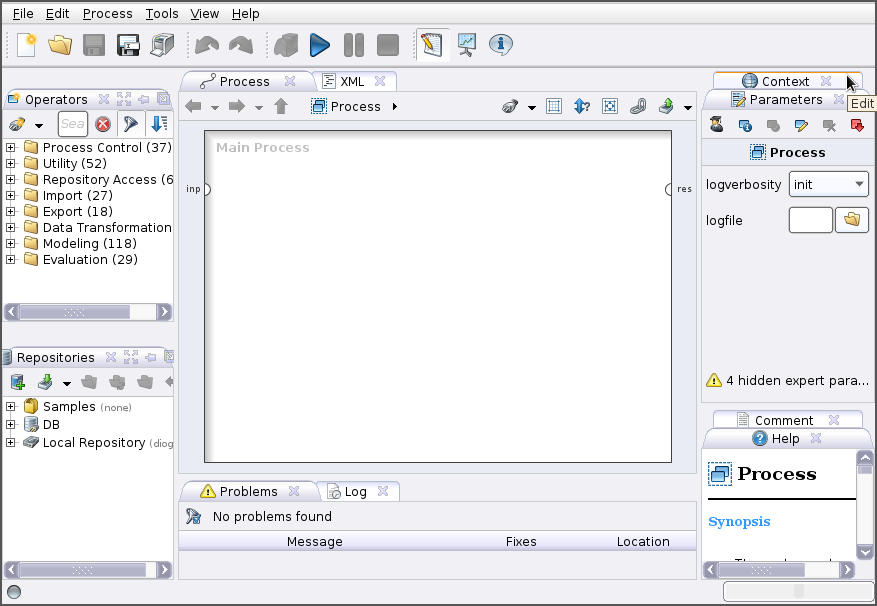
\includegraphics[width=0.6\textwidth]{rapidminer}
	\caption{RapidMiner's interface}
    \label{fig:rapidminer}
  \end{center}
\end{figure}

\subsubsection{WEKA}
Weka \footnote{WEKA: \url{http://www.cs.waikato.ac.nz/ml/weka/}} is an open source tool that collects several machine learning algorithms and allows its user to easily apply those algorithms to data mining tasks \cite{han2006data}. Created at the University of Waikato, New Zeland in 1997 (the current version was completely rewritten in 1997, despite the first iteration of the tool being developed as early as 1993), it's still in active development to date. Weka supports several common data mining tasks, like data preprocessing, classification, clustering, regression and data visualization. Its core libraries are written in Java and allow for an easy integration of its data mining algorithms in pre existing code and applications. Other than that, Weka can be used directly through a command line/terminal or through one of its multiple GUIs (Figure \ref{fig:weka}). Its simple API and well structure architecture allow it to be easily extended by users, should they need new functionalities.

\begin{figure}[htb]
  \begin{center}
    \leavevmode
    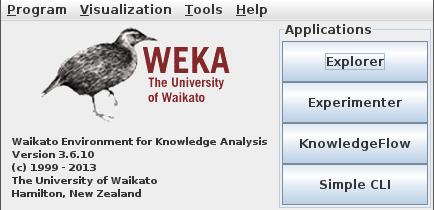
\includegraphics[width=0.6\textwidth]{weka}
	\caption{WEKA's interface}
    \label{fig:weka}
  \end{center}
\end{figure}

\subsubsection{R}
R \footnote{R: \url{http://www.r-project.org/}} is a free software environment for statistical computing and graphics. It compiles and runs on a wide variety of UNIX platforms, Windows and MacOS. R provides a wide variety of statistical (linear and nonlinear modeling, classical statistical tests, time-series analysis, classification, clustering, among others) and graphical techniques, and is highly extensible.  R is typically used by statisticians and data miners, either for direct data analysis or for developing new statistical software \cite{fox2005using}.\\
R is an open-source implementation of the S programming language, borrowing some characteristics from the Scheme programming language. Its core is written in a combination of C, Fortran and R itself. It is possible to directly manipulate R objects in languages like C, C++ and Java. R can be used directly through the command line or through several third party graphical user interfaces like Deducer \footnote{Deducer: http://www.deducer.org/pmwiki/index.php}. There are also R wrappers for several scripting languages.\\
R provides several different statistical and graphical techniques, including linear and nonlinear modeling, classical statistical tests, time-series analysis, classification, clustering, among others. It can also be used to produce publication-quality static graphics. Tools like Sweave \cite{leisch2002sweave} allow users to embed R code in \LaTeX documents, for complete data analysis.

\subsubsection*{arules}
The arules package \footnote{arules: \url{http://cran.r-project.org/web/packages/arules/index.html}} is a R package for mining association rules and frequent itemsets. Its sister package, arulesViz \footnote{http://cran.r-project.org/web/packages/arulesViz/index.html}, allows the visualization of the results found by arules. Since it is common to work with large sets of rules and itemsets, the package uses sparse matrix representations to minimize memory usage. The infrastructure provided by the package was also created to explicitly facilitate extensibility, both for interfacing new algorithms and for adding new types of interest measures and associations.

\subsubsection*{TraMineR}
TraMineR \footnote{TraMineR: \url{http://mephisto.unige.ch/traminer/}} (a contraction of Life Trajectory Miner for R) is a R-package for mining, describing and visualizing sequences of states or events, and more generally discrete sequential data. An example of the visualization features can be found in Figure \ref{fig:traminer}. Its primary aim is the analysis of biographical longitudinal data in the social sciences, such as data describing careers or family trajectories. Most of its features also apply, however, to non temporal data. TraMineR is developed at the Institute for Demographic and Life Course Studies (IDEMO), University of Geneva, Switzerland under the responsibility of the TraMineR Scientific Committee. 

\afterpage{
\begin{figure}[!htb]
  \begin{center}
    \leavevmode
    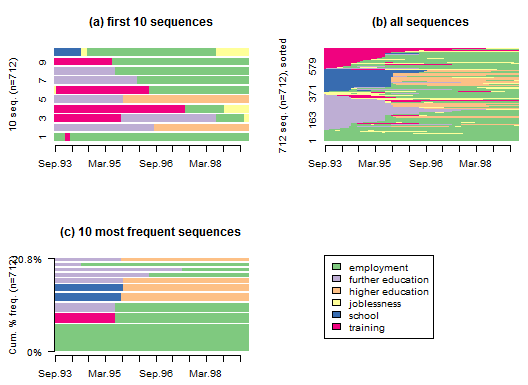
\includegraphics[width=0.8\textwidth]{traminer}
	\caption[An example of data visualization using TraMineR]{An example of data visualization using TraMineR\protect\footnotemark}
    \label{fig:traminer}
  \end{center}
\end{figure}
\footnotetext{Image extracted from: \url{http://mephisto.unige.ch/traminer/preview-visualizing.shtml}}
}

\subsubsection{SPMF (Sequential Pattern Mining Framework)}
SPMF \footnote{SPMF: \url{http://www.philippe-fournier-viger.com/spmf/}} is an open-source data mining library written in Java and distributed under the GPL v3 license. It includes implementations for sequential pattern mining, association rule mining, frequent itemset mining, sequential rule mining, and clustering algorithms, and has over 80 citations.

\section{Patterns}\label{sec:patterns}
User Interaction (UI) patterns are well-documented in a various number of sources \cite{tidwell2010designing,van2001patterns, neil12standard,sinnig2005patterns}. The patterns already supported (like the Search and Master/Detail patterns) enter the list of most popular patterns, according to the sources found, and if the selection of supported patterns were to be broadened, the pick of the next one(s) would be heavily influenced by the literature. Lin and Landay's approach \cite{lin2008employing} uses UI patterns for Web applications that run on PCs and mobile phones, and prompt-and-response style voice interfaces. Pontico \textit{et al.}'s approach \cite{pontico2008organizing} presents UI patterns common in eGovernment applications.

\section{Chapter Conclusions}
